\documentclass[british,10pt]{beamer}
\usepackage{pifont}
\usepackage{listings}
\usepackage{adjustbox} % for \adjincludegraphics

% Beamer specific settings

% Other styles can be used instead of Boadilla, e.g., to add an index column.
\mode<presentation>
{
  \usetheme{Boadilla} % Without index, with footer
}

\title{Building a better VHDL testing environment}
\author[J. Guillaume]{Joren Guillaume}
\date[JAN'15, Gent]{Thesis presentation}
\institute[Ghent University]
{
  FEA\\
  Ghent University
}

% This command makes the logo appear at the right side which does not fit
% the UGent style. A solution is found further below.
% \logo{\includegraphics[scale=0.25]{logolabel.jpg}}

\AtBeginSection[]
{
  \begin{frame}<beamer>\frametitle{Outline}
    \tableofcontents[currentsection,currentsubsection]
  \end{frame}
}

\setbeamersize{text margin left=1cm}
\setbeamersize{text margin right=1cm}

\begin{document}


% Titlepage containing the logo of the Faculty (Engineering in this example)
\begin{frame}[plain]
\mode<presentation>{
\includegraphics[width=\textwidth]{tw.pdf}}
  \titlepage
\end{frame}


% UGent logo at left side from second slide on.
\setbeamertemplate{sidebar left}{ 
\vfill 
\rlap{%\hskip0.1cm 
 
\includegraphics[scale=0.3]{logolabel2.jpg} } 
\vskip10pt 
}

\begin{frame}<beamer>\frametitle{Outline}
  \tableofcontents
\end{frame}




\section{Situating}
\subsection{Software development techniques}
\begin{frame}\frametitle{Software development techniques}
\begin{columns}
\begin{column}{0.6\textwidth}
Unit testing
\begin{itemize}
\item Unit = smallest behaviour in code
\item Test failure \ding{222} exact location
\end{itemize}
\vskip3pt
Test First Development
\begin{itemize}
\item Create test before the code
\item How will the code behave?
\end{itemize}
\vskip3pt
Test Driven Development
\begin{itemize}
\item TFD \& refactoring
\item Proven to significantly reduce errors
\end{itemize}
\end{column}
\column{0.4\textwidth}
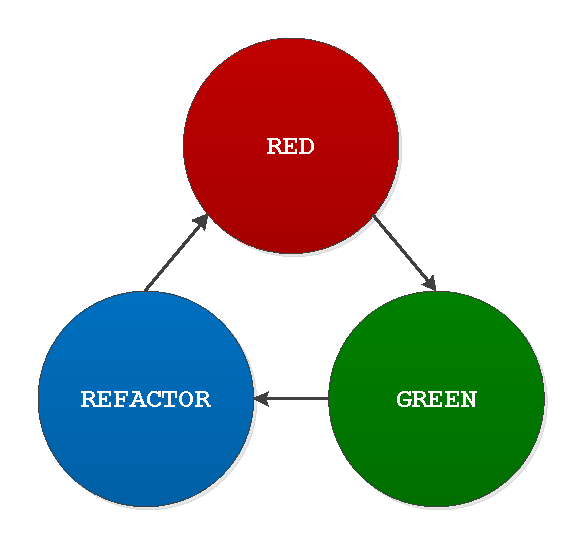
\includegraphics[width=\textwidth]{images/tdd.pdf}
\end{columns}
\end{frame}


\subsection{VHDL}
\begin{frame}\frametitle{VHDL}
\begin{itemize}
\item VHSIC Hardware Description Language
\item Used for describing digital and mixed-signal systems 
\item Developed by U.S. Department of Defense
\begin{itemize}
\item Document \ding{222} Simulate \ding{222} Synthesize
\end{itemize}
\end{itemize}
\end{frame}

\subsection{Testing and problems}

\begin{frame}\frametitle{Testing VHDL}
\begin{columns}
\begin{column}{0.05\textwidth}
\end{column}
\begin{column}{0.55\textwidth}
Test benches
\begin{itemize}
\item Unit Under Test (UUT)
\item Apply stimuli
\item Signal/output tracking
\begin{itemize}
\item Assertions
\item Comparison to desired result
\item Wave-check
\end{itemize}
\end{itemize}
%\vspace{0.25cm}
%Problems
%\begin{itemize}
%\item Non-standardized process
%\item Single point of failure
%\item Time consuming
%\end{itemize}
\end{column}
\column{0.4\textwidth}
\raggedleft
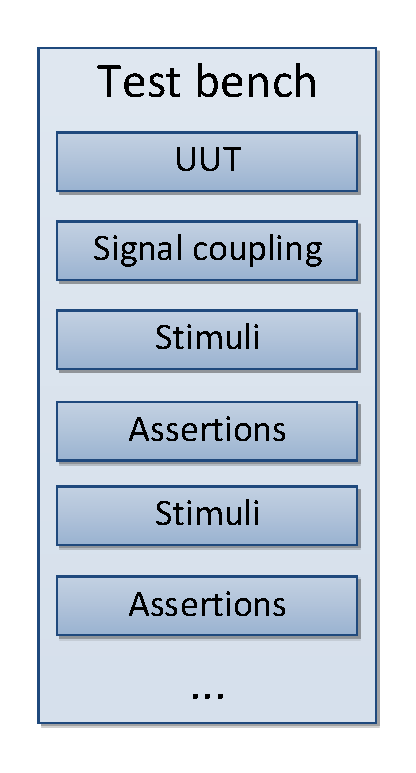
\includegraphics[width=\textwidth]{images/TB.pdf}
\end{columns}
\end{frame}

\begin{frame}\frametitle{Testing VHDL}
Problems with testing
\begin{itemize}
\item Non-standardized process
\item Single point of failure
\item Time consuming
\end{itemize}
\end{frame}


\section{Proposed solution}
\begin{frame}\frametitle{Proposed solution}
Apply unit testing to VHDL?
\begin{itemize}
\item[=] 1 unit test per test bench
\begin{itemize}
\item[\ding{222}] Extremely large number of TBs
\item[\ding{222}] Impractical, time wasting
\end{itemize}
\end{itemize}
\vskip5pt
Solution: have a framework do it for you
\end{frame}

\subsection{VHDL testing framework}
\begin{frame}\frametitle{VHDL testing framework}
%\vskip20pt
\begin{columns}
\begin{column}{0.65\textwidth}
\begin{enumerate}
\item Arrange tests into unit tests (test suite)
\item Separate unit tests into files
\item Compile source and newly created files
\item Execute unit tests
\item Capture and process results
\end{enumerate}
\end{column}
\column{0.05\textwidth}
\vskip12pt
\Huge\}
\vskip1pt
\}
\column{0.25\textwidth}
\ding{222} Prepare
\vskip13pt
\ding{222} Process
\vskip17pt
\ding{222} Execute
\end{columns}
%\vskip20pt
%\centering
%
\includegraphics[width=.7\textwidth]{images/ppe.pdf}
\end{frame}

\begin{frame}\frametitle{VHDL testing framework}
\vskip45pt
Python script + ModelSim
\vskip10pt
\begin{itemize}
\item Prepare
\begin{itemize}
\item[\ding{222}] Developer arranges test suite
\end{itemize}
\item Process
\begin{itemize}
\item[\ding{222}] Python script separates unit tests
\item[\ding{222}] ModelSim compiles all files
\end{itemize}
\item Execute
\begin{itemize}
\item[\ding{222}] ModelSim executes unit tests
\item[\ding{222}] Python script reads output
\end{itemize}
\end{itemize}
\vskip45pt
\begin{center}

\includegraphics[width=.7\textwidth]{images/ppe.pdf}
\end{center}
\end{frame}


\subsection{Using the framework}
\begin{frame}[fragile]\frametitle{Preparing test benches}
\vskip25pt
\begin{itemize}
\item Separate independent tests
\begin{itemize}
\item Line by line
\item Start/Stop
\item Partitioned
\end{itemize}
\begin{lstlisting}[language=VHDL, tabsize=4, frame=single, framesep=2mm, belowskip=5pt, aboveskip=5pt, showstringspaces=false, basicstyle=\scriptsize]
...
--Test 1
assert q = '0'
    report "Wrong output value at startup" severity FAILURE;
d <= '1';
WAIT FOR clk_period;
assert q = '1'
    report "Wrong output value at first test" severity FAILURE;
--End 1
...
\end{lstlisting}
\item Create commands file
\end{itemize}
\vskip15pt
\begin{center}

\includegraphics[width=.7\textwidth]{images/ppe1.pdf}
\end{center}
\end{frame}

\begin{frame}[fragile]\frametitle{Utility library}
\vskip30pt
\begin{columns}
\begin{column}{0.6\textwidth}
Use Bitvis utility library for:
\begin{itemize}
\item Faster coding
\item Improved readability
\end{itemize}
%\hskip24pt\ding{222} Unit testing
\end{column}
\column{0.4\textwidth}

\includegraphics[width=0.8\textwidth]{images/bitvis.png}
\end{columns}
\vskip10pt
Modified unit test:
\begin{lstlisting}[language=VHDL, tabsize=4, frame=single, framesep=2mm, belowskip=5pt, aboveskip=5pt, showstringspaces=false, basicstyle=\scriptsize]
...
--Test 1
    check_value(q = '0', FAILURE, "Wrong output value at startup");
    write(d, '1', "DFF");
    check_value(q = '1', FAILURE, "Wrong output value at first test");
--End 1
...
\end{lstlisting}
\vskip30pt
\begin{center}

\includegraphics[width=.7\textwidth]{images/ppe1.pdf}
\end{center}
\end{frame}

%\subsection{Using the framework}
%\begin{frame}\frametitle{Preparing test benches}
%\vskip50pt
%\begin{columns}
%\begin{column}{0.6\textwidth}
%\begin{itemize}
%\item Use Bitvis utility library
%\begin{itemize}
%\item Faster coding
%\item Improved readability
%\end{itemize}
%\item Separate independent tests
%\begin{itemize}
%\item Line by line
%\item Start/Stop
%\item Partitioned
%\end{itemize}
%\item Create commands file
%\end{itemize}
%%\hskip24pt\ding{222} Unit testing
%\end{column}
%\column{0.4\textwidth}
%
\includegraphics[width=0.8\textwidth]{images/bitvis.png}
%\end{columns}
%\centering
%\vskip50pt
%
\includegraphics[width=.7\textwidth]{images/ppe1.pdf}
%\end{frame}
%
%\begin{frame}[fragile]\frametitle{Modified test bench example}
%D flip-flop
%\begin{itemize}
%\item Old test bench:
%\end{itemize}
%\begin{lstlisting}[language=VHDL, tabsize=4, frame=single, framesep=2mm, belowskip=5pt, aboveskip=5pt, showstringspaces=false, basicstyle=\scriptsize]
%assert q = '0'
%    report "Wrong output value at startup" severity FAILURE;
%d <= '1';
%WAIT FOR clk_period;
%assert q = '1'
%    report "Wrong output value at first test" severity FAILURE;
%\end{lstlisting}
%\vskip1pt
%\begin{itemize}
%\item Modified test bench:
%\end{itemize}
%\begin{lstlisting}[language=VHDL, tabsize=4, frame=single, framesep=2mm, belowskip=5pt, aboveskip=5pt, showstringspaces=false, basicstyle=\scriptsize]
%--Test 1
%    check_value(q = '0', FAILURE, "Wrong output value at startup");
%    write(d, '1', "DFF");
%    check_value(q = '1', FAILURE, "Wrong output value at first test");
%    ...
%--End 1
%\end{lstlisting}
%\end{frame}


\begin{frame}\frametitle{Processing and compiling}
\vskip20pt
Python script:
\begin{itemize}
\item Reads command line arguments
\item Reads test suite
\item Separates test suite into unit tests
\end{itemize}
\vskip5pt
\centering
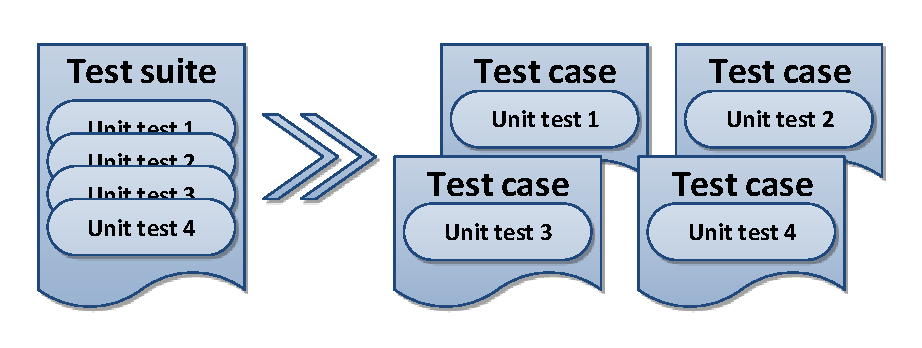
\includegraphics[width=.8\textwidth]{images/tbsplit2.pdf}
\vskip20pt

\includegraphics[width=.7\textwidth]{images/ppe2.pdf}
\end{frame}



%\begin{frame}\frametitle{Proposed solution}
%Standardized testing framework
%\begin{itemize}
%\item Based on unit testing
%\item Cross platform
%\item At the core: Python script
%\item Utility library
%\item Continuous Integration system
%\end{itemize}
%\end{frame}
%\subsection{VHDL testing framework}

\begin{frame}\frametitle{Processing and compiling}
\vskip30pt
ModelSim:
\begin{itemize}
\item Compiles source code (UUT)
\item Compiles test suite
\begin{itemize}
\item[\ding{222}] One entity, many architectures
\end{itemize}
\end{itemize}
\centering
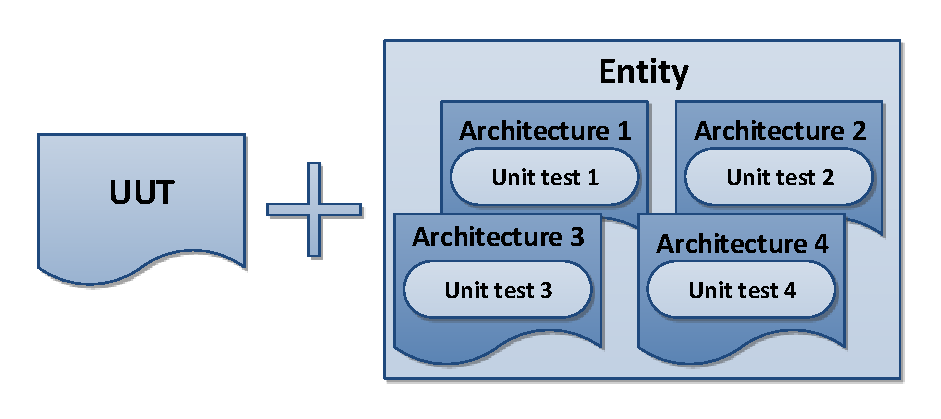
\includegraphics[width=.75\textwidth]{images/sources2.pdf}
\vskip10pt

\includegraphics[width=.7\textwidth]{images/ppe2.pdf}
\end{frame}


\begin{frame}\frametitle{Execution and results}
\vskip48pt
ModelSim:
\begin{itemize}
\item Executes each unit test
\end{itemize}
\vskip5pt
Python script:
\begin{itemize}
\item Captures ModelSim output
\item Processes results
\begin{itemize}
\item Text report
\item JUnit XML report
\end{itemize}
\end{itemize}
\centering
\vskip48pt

\includegraphics[width=.7\textwidth]{images/ppe3.pdf}
\end{frame}

\subsection{Automation}
\begin{frame}\frametitle{Automation}
\begin{columns}
\begin{column}{0.6\textwidth}
Hudson-CI
\begin{itemize}
\item Gets latest version from RC
\begin{itemize}
\item Timed retrieval
\item Detect changes
\end{itemize}
\item Automated script execution
\item Result progress (XML)
\end{itemize}
\end{column}
\column{0.4\textwidth}

\includegraphics[width=0.8\textwidth]{images/hudson.png}
\end{columns}
\end{frame}

\section{Concluding}

\subsection{Results}
\begin{frame}\frametitle{Results}
Multiple open-source projects tested
\vskip10pt
{\centering
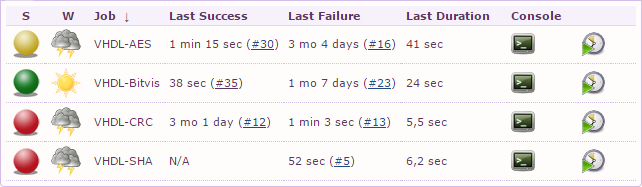
\includegraphics[width=\textwidth]{images/jobs.png}}
%\\\hskip10pt\ding{222} Bypassed single point of failure
%\\\hskip10pt\ding{222} Automated testing = faster development
%\\\hskip10pt\ding{222} Successful runs when VHDL code OK
%\\\hskip10pt\ding{222} Partially completed test-runs even with faults in code
%\\\hskip10pt\ding{222} Unsuccessful runs only due to compilation errors\\
\end{frame}


\begin{frame}\frametitle{Results}
Precise debugging information
{\centering
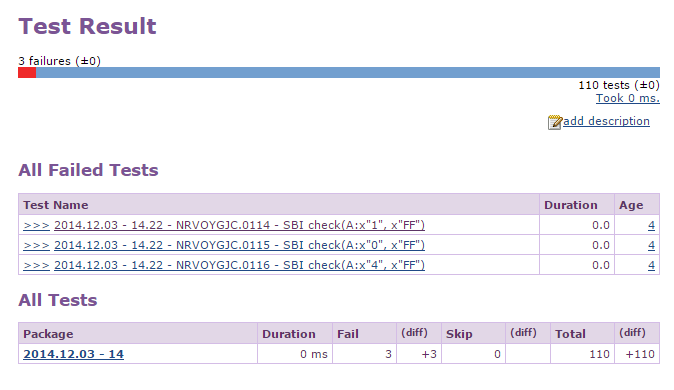
\includegraphics[width=.95\textwidth]{images/results1.png}}
\end{frame}
\subsection{Future work}

\begin{frame}\frametitle{Future work}
\begin{itemize}
\item Wider, better tool support
\item Lexical analysis
\begin{itemize}
\item Automated unit test recognition
\item Smart testsuite generation
\end{itemize}
\item Adapted CI tool
\begin{itemize}
\item Specific needs of hardware development
\end{itemize}
\end{itemize}
\end{frame}
%%VOLGENDE
%%STAP
%%IN
%%DEZE
%%ONTWIKKELING
%%WAT
%%NU?

\subsection{Conclusion}

\begin{frame}\frametitle{Conclusion}
\begin{itemize}
\item Software methods are applicable if:
\begin{itemize}
\item Tailored to development needs
\item Integrated with existing methods
\end{itemize}
\vskip3pt
\item The framework provided:
\begin{itemize}
\item Easier to read code
\item Precise debugging information
\item Eliminated single point of failure
\end{itemize}
\end{itemize}
\end{frame}


\begin{frame}\frametitle{End}
\centering
\Large
Thanks for your attention!
\vskip20pt
Questions?
\end{frame}

\section{Demo}
\begin{frame}\frametitle{Demo}
\centering
\Huge Demo
\end{frame}

\end{document}
